%
% IT.
% Information Technology
%
% Aleph Objects Operations Manual
%
% Copyright (C) 2014, 2015 Aleph Objects, Inc.
%
% This document is licensed under the Creative Commons Attribution 4.0
% International Public License (CC BY-SA 4.0) by Aleph Objects, Inc.
%

\section{Network}
The Aleph Objects network is comprised of workstations, phones and servers at
Aleph Mountain and our upstream providers. See figure
\ref{fig:ao_net_overview} for an overview of Aleph Objects' network,
figure \ref{fig:ao_net_sfdp} for a detailed network diagram, and
figure \ref{fig:ao_net_dia} for an older network diagram.

\begin{figure}[h!]
% The ao-network-overview.pdf built in calligraflow.
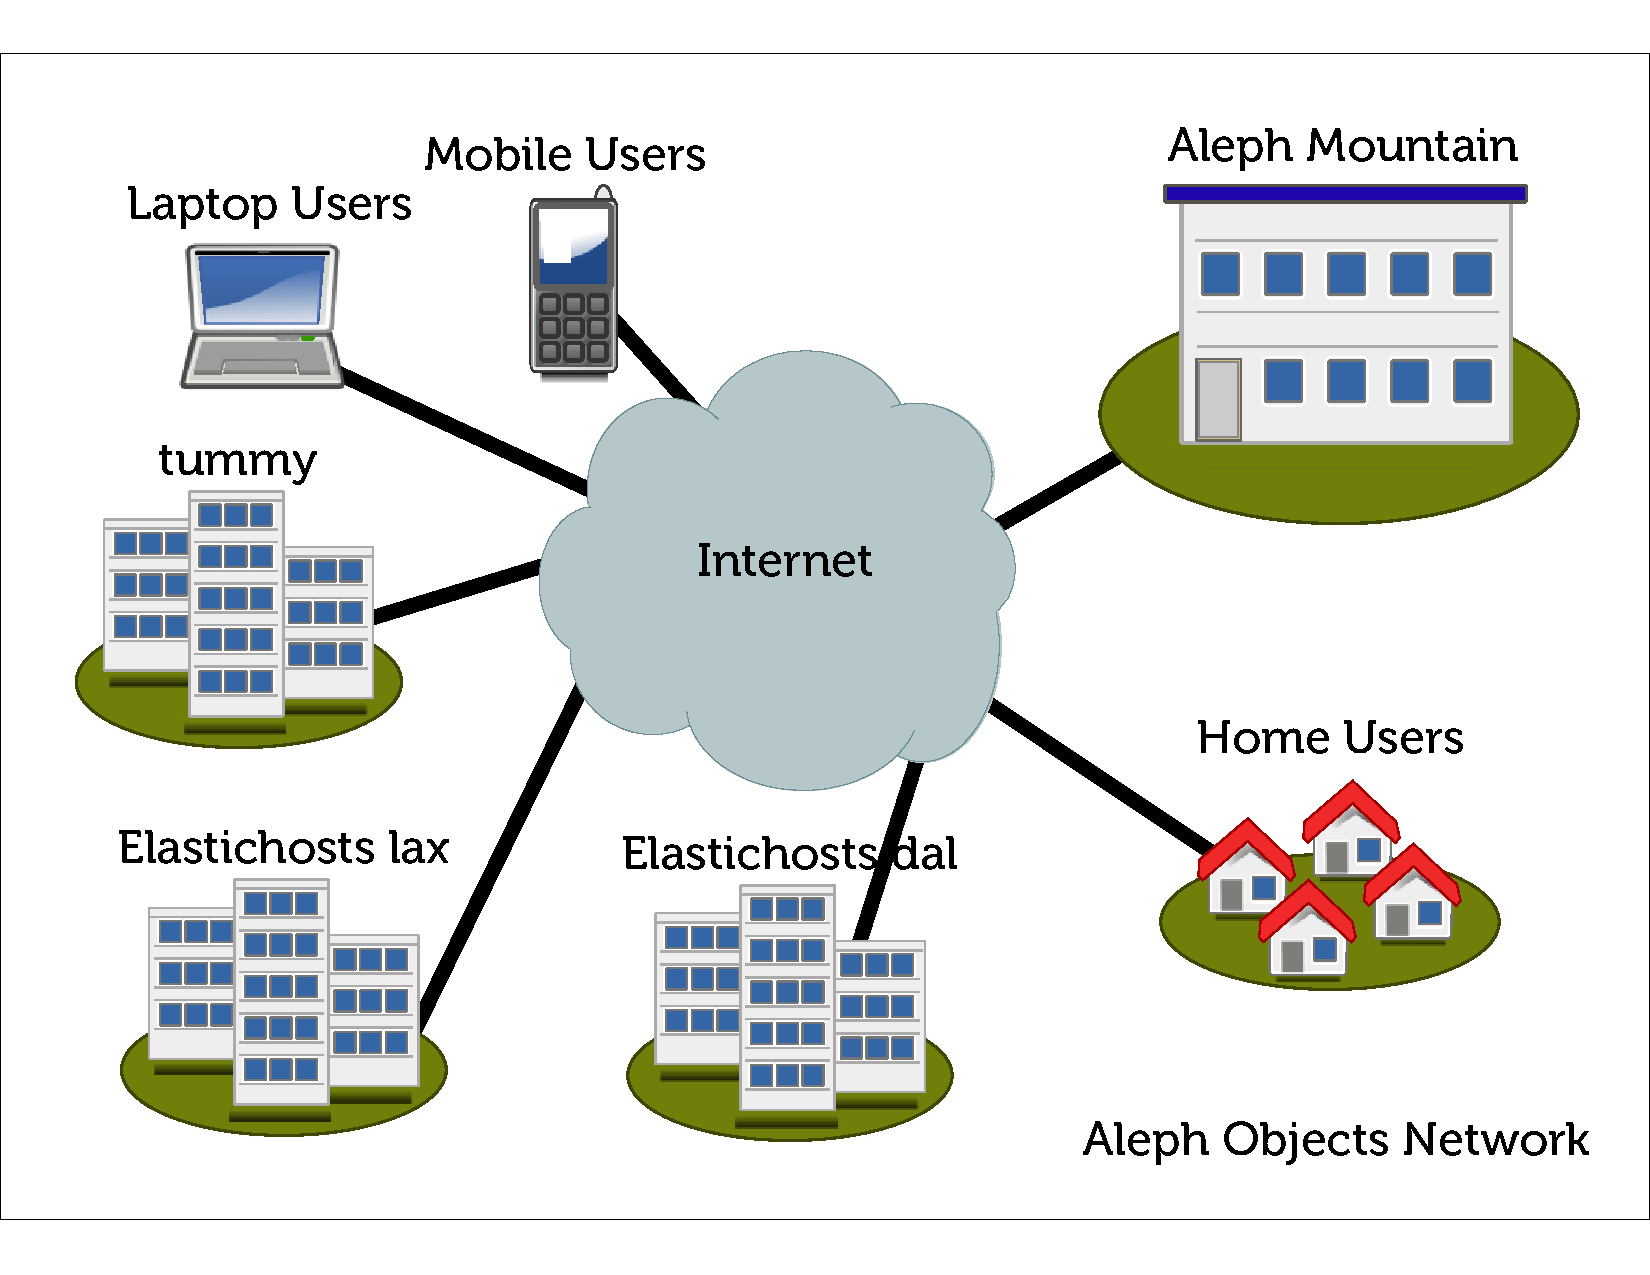
\includegraphics[keepaspectratio=true,height=1.10\textheight,width=1.00\textwidth,angle=0]{ao-network-overview.pdf}
 \caption{Aleph Objects Network Overview, May, 2015}
 \label{fig:ao_net_overview}
\end{figure}

\section{Servers}
In general, the servers are all running the latest stable release of Debian,
Jessie, version 8, on the amd64 architecture. Some are running Wheezy because
the daemon they hosts prefers it. There is some Debian Squeeze, which is being
migrated. The firewalls are OpenBSD. There is one CentOS and one Fedora
machine.

All machines are backed up at least daily. Updates are run at least weekly,
sooner depending on the nature of the update.

\subsection{Aleph Mountain Servers}
This is a list of servers and nodes that are in the Aleph Mountain building.

\begin{itemize}
\item \texttt{abejas.alephobjects.com} --- Apache, OpenERP.
\item \texttt{amfw1.alephobjects.com} --- OpenBSD, PF, authpf.
\item \texttt{amfw2.alephobjects.com} --- OpenBSD, PF.
\item \texttt{aobuild1.alephobjects.com} --- Compile/build server.
\item \texttt{aocluster1.alephobjects.com} --- 3D Printer cluster Botqueue
       server.
\item \texttt{aodb.alephobjects.com} --- Postgres.
\item \texttt{aogfs1.alephobjects.com} --- Test, potential fileserver.
\item \texttt{aomds1.alephobjects.com} --- Test, potential db server.
\item \texttt{cam.alephobjects.com} --- Motion, Motioneye video camera server.
\item \texttt{jebstation.alephobjects.com} --- sshfs file server.
\item \texttt{tunk.alephobjects.com} --- apt-cacher, OpenVPN server, dnsmasq
      (dhcp, dns cache, tftp), MySQL, OpenLDAP.
\end{itemize}

\subsection{Virtual Servers Elastichosts Los Angeles}
These are machines ``in the cloud''.

\begin{itemize}
\item \texttt{aomail.alephobjects.com} --- Apache, Roundcube.
\item \texttt{analytics.alephobjects.com}  --- Apache, Piwik, MySQL.
\item \texttt{cal.alephobjects.com} --- Calendarserver.
\item \texttt{develdrupal.lulzbot.com} --- Test server. Apache, Drupal,
       Ubercart, MySQL.
\item \texttt{develerp.alephobjects.com} --- Test server. OpenERP, Postgres.
\item \texttt{dodev.alephobjects.com} --- Test server. Odoo, Postgres.
\item \texttt{drupalsql.lulzbot.com} --- MySQL.
\item \texttt{drupalsqlslave.lulzbot.com} --- MySQL, Offline.
\item \texttt{forum.lulzbot.com} --- Apache, phpBB, MySQL.
\item \texttt{jabber.alephobjects.com} --- ejabberd.
\item \texttt{ldap.alephobjects.com} --- OpenLDAP.
\item \texttt{ohai-kit.alephobjects.com} --- Apache, OHAI-Kit, MySQL.
\item \texttt{ops.alephobjects.com} --- Apache, Opsview.
\item \texttt{phplist.alephobjects.com} --- Apache, phplist.
\item \texttt{projects.alephobjects.com} --- Apache, OpenProjects, MySQL.
\item \texttt{survey.alephobjects.com} --- Apache, LimeSurvey.
\item \texttt{thinkup.alephobjects.com} --- Apache, ThinkUp, MySQL, Offline.
\item \texttt{www.lulzbot.com} --- Apache, Drupal, Ubercart.
\item \texttt{www.alephobjects.com} --- Apache, HTML.  :)
\end{itemize}

\subsection{Virtual Servers Elastichosts Dallas}
These are machines ``in the cloud''.

\begin{itemize}
\item \texttt{download.alephobjects.com} --- Apache, vsftpd, rsyncd.
\item \texttt{fone.alephobjects.com} --- Asterisk.
\item \texttt{mail.alephobjects.com} --- Postfix, dovecot, spamassassin, MySQL.
\item \texttt{wiki.alephobjects.com} --- Test server. Apache, Mediawiki, MySQL.
\end{itemize}

\subsection{Tummy Servers}
The CentOS server at Tummy.

\begin{itemize}
\item \texttt{belly1.alephobjects.com} --- Tummy Backup server.
\end{itemize}

\section{Public Services}
\subsection{Public URLs}
\begin{itemize}
\item \url{https://www.alephobjects.com} --- Main Aleph Objects website.
\item \url{https://www.lulzbot.com} --- Main LulzBot website.
\item \url{https://devel.alephobjects.com} --- Public development files for
       Aleph Objects.
\item \url{https://devel.lulzbot.com} --- Public development files for LulzBot.
\item \url{https://download.alephobjects.com} --- Aleph Objects downloads.
\item \url{https://download.lulzbot.com} --- Final release source code for
       LulzBot products.
\item \url{https://forum.lulzbot.com} --- User discussion forum for LulzBot.
\item \url{https://ohai-kit.alephobjects.com} --- Visual work instructions for
       assembling products and user support.
\item \url{https://phplist.alephobjects.com} --- Newletter mailing list.
\item \url{https://survey.alephobjects.com} --- Surveys.
\item \url{rsync://rsync.alephobjects.com} --- Rsync file server of download
       and development archives.
\end{itemize}

\section{Employee Services}
\subsection{Employee URLs}
These are URLs that are for Aleph Objects employees.

\begin{itemize}
\item \url{https://analytics.alephobjects.com} --- Website analytics.
\item \url{https://aomail.alephobjects.com} --- Webmail server.
\item \url{https://belly1.alephobjects.com} --- Backup server.
\item \url{https://erp.alephobjects.com} --- ERP server.
\item \url{https://ops.alephobjects.com} --- Network monitoring.
\item \url{https://projects.alephobjects.com} --- Project tracking.
\item \url{https://wiki.alephobjects.com} --- Development wiki.
\end{itemize}

\section{Server Daemons}
These are the server daemons used to drive the enterprise.

\subsection{\href{http://sourceforge.net/projects/acpid2/}{ACPID}}
Monitors ACPI events. Runs on nearly all servers and workstations.

\subsection{\href{http://httpd.apache.org/}{Apache}}
Web daemon, used on many servers.

\subsection{\href{http://www.asterisk.org}{Asterisk}}
Telephone server. DIDs (incoming), termination (outgoing), forwarding of calls, conferencing,
voicemail, XMPP.

\subsection{\href{https://github.com/tummy-dot-com/tummy-backup}{Backups}}
tummy-backup backup server.

\subsection{\href{http://www.isc.org/}{BIND}}
Nameserver used for caching.

\subsection{\href{http://www.botqueue.org/}{botqueue}}
Print queue manager.

\subsection{\href{http://www.debian.org/}{buildd}}
Build service for compiling Debian packages.

\subsection{\href{http://www.calendarserver.org/}{Calendar Server}}
Calendar (CalDAV) and contacts (CardDAV) server. CalDAV is used with mobile
phones and icedove. No group calendars. CardDav is unused. Uses python-twisted.

Needs to be connected to or replaced by LDAP.

\subsection{\href{http://ftp.isc.org/isc/cron/}{cron}}
Scheduled triggering of applications (cf. at).

\subsection{\href{http://dnsmasq.org/}{DHCP}}
dnsmasq DHCP for 350+ hosts.

\subsection{\href{http://dnsmasq.org/}{DNS}}
dnsmasq DNS caching.

\subsection{\href{http://dnsmasq.org/}{Dovecot}}
IMAP mail services. Employees check their mail via the
IMAP server, typically using icedove or aomail (roundcube using IMAP).

\subsection{\href{http://www.drupal.org}{Drupal}}
Main LulzBot site.

Used with \href{http://www.ubercart.org/}{UberCart}.
Migrating to Drupal Commerce.

\subsection{\href{http://www.exim.org/}{exim}}
SMTP outgoing mail server, used by default in Debian. Used by some servers.

\subsection{\href{http://www.openbsd.org/faq/pf/}{Firewalls}}
OpenBSD's PF, authpf, Linux's iptables.

\subsection{\href{http://www.fail2ban.org/}{fail2ban}}
Block out scripts, bots, crackers, and network noise on servers.

\subsection{\href{http://www.debian.org/}{Init}}
Init, woo!

\subsection{md RAID}
Linux RAID, md, mdadm.

\subsection{\href{http://www.mediawiki.org/}{Mediawiki}}
Test/development server for customer support.

\subsection{\href{http://www.memcached.org/}{memcached}}
Used to speed up websites, such as Drupal.

\subsection{\href{http://motion.sf.net}{Motion}}
Motion detection for video camera system. Cameras are aggregated
using \href{https://bitbucket.org/ccrisan/motioneye/wiki/Home}{motionEye}.

\subsection{\href{http://munin-monitoring.org/}{Munin}}
Network graphing.

\subsection{\href{http://www.mysql.org/}{MySQL}}
Used on many servers for a database.

\subsection{\href{http://support.ntp.org/}{NTP}}
Syncs time on every server and workstation.

\subsection{\href{http://www.odoo.com/}{Odoo}}
Development ERP server, next generation of OpenERP.

\subsection{\href{http://www.openerp.org/}{OpenERP}}
ERP server.

\subsection{\href{http://www.openldap.org/}{OpenLDAP}}
LDAP server. Running, but not actively used. Daemon is slapd.

\subsection{\href{http://www.openssh.com/}{OpenSSH}}
Used to control every server, create encrypted tunnels (autossh),
mount filesystems (sshfs), and remote file transfer (sftp).

\subsection{\href{http://openvpn.net/}{OpenVPN}}
Connects external resources, such as employee mobiles and laptops, to the internal network.

\subsection{\href{http://www.opsview.com/}{Opsview}}
Network monitoring (cf. nagios).

\subsection{\href{http://community.pentaho.com/}{Pentaho}}
Report server, connects to ERP.

\subsection{\href{https://www.piwiki.org/}{Piwik}}
Application to analyze web site traffic.

\href{http://www.mrunix.net/webalizer/}{Webalizer} is used occassionally.

\subsection{\href{https://www.phpbb.com/}{phpBB}}
User discussion forum.

\subsection{\href{http://www.postfix.org/}{Postfix}}
Main SMTP outgoing mail server.

\subsection{\href{http://www.postgresql.org/}{Postgres}}
Database server.

\subsection{\href{http://rsync.samba.org/}{rsync}}
File server.

\subsection{\href{http://www.rsyslog.com/}{rsyslog}}
Logging on every server and workstation.

\subsection{\href{http://www.openbsd.org/cgi-bin/man.cgi/OpenBSD-current/man8/sendmail.8?query=sendmail&sec=8}{sendmail}}
SMTP outgoing mail server, used by default in OpenBSD.

\subsection{\href{http://www.spamassassin.org/}{spamassassin}}
Spam filtering of email.

\subsection{\href{http://fuse.sourceforge.net/sshfs.html}{sshfs}}
Main internal fileserver.

\subsection{\href{http://www.freedesktop.org/wiki/Software/systemd}{systemd}}
System bootup and process manager.

\subsection{\href{http://dnsmasq.org/}{TFTP}}
Network install server.

\subsection{\href{http://vsftpd.beasts.org/}{vsftpd}}
vsftpd FTP server for public facing download and devel servers.

\subsection{\href{http://www.xinetd.org}{xinetd}}
xinetd on Debian systems. inetd on OpenBSD. Misc network utils.

\subsection{\href{http://www.ejabberd.im/}{XMPP/jabber}}
ejabberd, Erlang XMPP (jabber) server.


\section{3D Printer Cluster}
There are 144 printers in the 3D printing cluster. One hundred thirty five are
in the main cluster room, nine in the adjoining sample room. The cluster is a
mix of LulzBot TAZ and LulzBot Minis.

Each printer has a Beaglebone Black (BBB) connected to it via USB. The
BBB is running Debian (armhf port) and Botqueue. There is a separate Botqueue
server, also running Debian, that the BBBs connect to, to get print jobs.

The printers are organized in sets, or ``pods'', typically of nine. Each cabinet
holds nine machines, three wide by three high. Each pod is assigned a letter.
In the main cluster room, this is A through O. In the sample room, it is pods
Y and Z which have five and four machines, respectively. Machines are named
of the format: bbb-a1, bbb-a2, through to bbb-a9 for the first pod. Then the
next pod starts bbb-b1, through to the end: bbb-z4.

List of printers:
\begin{itemize}
\item \texttt{bbb-a1.alephobjects.com} through
      \texttt{bbb-o9.alephobjects.com} --- LulzBot TAZ.
\item \texttt{bbb-y1.alephobjects.com} through
      \texttt{bbb-z4.alephobjects.com} --- LulzBot Mini.
\end{itemize}

Links to upstream:
\begin{itemize}
\item \href{http://beagleboard.org/}{BeagleBone Black}
\item \href{http://botqueue.org/}{BotQueue}
\item \href{https://wiki.debian.org/ArmHardFloatPort}{Debian armhf}
\end{itemize}

\section{Workstation Software}

All workstations run \href{http://www.debian.org/}{Debian} stable, version 8,
codename \href{https://www.debian.org/releases/jessie/}{Jessie}.

\subsection{Graphical User Interface (GUI) Applications}
\subsection{\href{http://christian.amsuess.com/tools/arandr/}{arandr}}

 ARandR is a visual front end for XRandR 1.2/1.3 (per display options), which
 provides full control over positioning, saving and loading to/from shell
 scripts and easy integration with other applications.

\subsection{\href{http://www.arduino.cc}{arduino}}

 Arduino is an open-source electronics prototyping platform based on
 flexible, easy-to-use hardware and software. It's intended for artists,
 designers, hobbyists, and anyone interested in creating interactive
 objects or environments.
 
 This package will install the integrated development environment that
 allows for program writing, code verfication, compiling, and uploading
 to the Arduino development board. Libraries and example code will also
 be installed.

\subsection{\href{http://audacity.sourceforge.net/}{audacity}}

 Audacity is a multi-track audio editor for Linux/Unix, MacOS and
 Windows.  It is designed for easy recording, playing and editing of
 digital audio.  Audacity features digital effects and spectrum
 analysis tools.  Editing is very fast and provides unlimited
 undo/redo.
 
 Supported file formats include Ogg Vorbis, MP2, MP3, WAV, AIFF, and AU.

\subsection{\href{http://www.blender.org/}{blender}}

 Blender is an integrated 3d suite for modelling, animation, rendering,
 post-production, interactive creation and playback (games). Blender has its
 own particular user interface, which is implemented entirely in OpenGL and
 designed with speed in mind. Python bindings are available for scripting;
 import/export features for popular file formats like 3D Studio and Wavefront
 Obj are implemented as scripts by the community. Stills, animations, models
 for games or other third party engines and interactive content in the form of
 a standalone binary are common products of Blender use.

\subsection{\href{http://www.chromium.org/Home}{chromium}}

 Web browser that aims to build a safer, faster, and more stable internet
 browsing experience.
 
 This package contains the web browser component.

\subsection{\href{}{cura}}

 aimed at Open Hardware 3D Printers. Cura is free software paid for
 and maintained by Ultimaker. Cura LulzBot Edition been modified and maintained by Aleph Objects, Inc. for use with LulzBot 3D printers.

\subsection{\href{http://www.darktable.org/}{darktable}}

 Darktable manages your digital negatives in a database and lets you view
 them  through a zoomable lighttable. it also enables you to develop raw
 images and enhance them.
 
 It tries to fill the gap between the many excellent existing free
 raw converters and image management tools (such as ufraw or f-spot).
 The user interface is built around efficient caching of image metadata and
 mipmaps, all stored in a database. the user will always be able to interact,
 even if the full resolution image is not yet loaded.
 
 All editing is fully non-destructive and only operates on cached image
 buffers for display. the full image is only converted during export. The
 frontend is written in gtk+/cairo, the database uses sqlite3, raw image
 loading is done using libraw, high-dynamic range, and standard image formats
 such as jpeg are also supported. The core operates completely on floating
 point values, so darktable can not only be used for photography but also for
 scientifically acquired images or output of renderers (high dynamic range).

\subsection{\href{http://live.gnome.org/Dia}{dia}}

 Dia is an editor for diagrams, graphs, charts etc. There is support for UML
 static structure diagrams (class diagrams), Entity-Relationship diagrams,
 network diagrams and much more. Diagrams can be exported to postscript and
 many other formats.

\subsection{\href{https://wiki.gnome.org/Apps/Web}{epiphany-browser}}

 Epiphany is a simple yet powerful GNOME web browser targeted at
 non-technical users. Its principles are simplicity and standards
 compliance.
 
 Simplicity is achieved by a well designed user interface and reliance
 on external applications for performing external tasks (such as reading
 email). Simplicity does not mean less features; Epiphany has everything
 a modern web browser is expected to have.
 
 Standards compliance is achieved on the HTML side by using the
 WebKitGTK+ rendering engine (which is based on the engine used by
 Apple Safari and Google Chrome); and on the user interface side by
 closely following the GNOME Human Interface Guidelines (HIG) and by
 close integration with the GNOME desktop.

\subsection{\href{https://wiki.gnome.org/Apps/Evince}{evince}}

 Evince is a simple multi-page document viewer.  It can display and print
 PostScript (PS), Encapsulated PostScript (EPS), DjVu, DVI, Portable
 Document Format (PDF) and XML Paper Specification (XPS) files.
 When supported by the document, it also allows searching for text,
 copying text to the clipboard, hypertext navigation, and
 table-of-contents bookmarks.

\subsection{\href{http://fileroller.sourceforge.net/}{file-roller}}

 File-roller is an archive manager for the GNOME environment. It allows you to:
 
  * Create and modify archives.
  * View the content of an archive.
  * View a file contained in an archive.
  * Extract files from the archive.
 
 File-roller supports the following formats:
  * Tar (.tar) archives, including those compressed with
    gzip (.tar.gz, tgz), bzip (.tar.bz, tbz), bzip2 (.tar.bz2, tbz2),
    compress (.tar.Z, taz), lzip (.tar.lz, tlz), lzop (.tar.lzo, tzo),
    lzma (.tar.lzma) and xz (.tar.xz)
  * Zip archives (.zip)
  * Jar archives (.jar, ear, war)
  * 7z archives (.7z)
  * iso9660 CD images (.iso)
  * Lha archives (.lzh)
  * Archiver archives (.ar)
  * Comic book archives (.cbz)
  * Single files compressed with gzip (.gz), bzip (.bz), bzip2 (.bz2),
    compress (.Z), lzip (.lz), lzop (.lzo), lzma (.lzma) and xz (.xz)
 
 File-roller can extract following formats:
  * Cabinet archives (.cab)
  * Debian binary packages (.deb)
  * Xar archives (.xar)
 
 File-roller doesn't perform archive operations by itself, but relies on
 standard tools for this.

\subsection{\href{http://freecadweb.org/}{freecad}}

 FreeCAD is an Open Source CAx RAD based on OpenCasCade, Qt and Python.
 It features some key concepts like macro recording, workbenches, ability
 to run as a server and dynamically loadable application extensions and
 it is designed to be platform independent.
 
 Currently, FreeCAD can import and display CAD models in IGES, STEP, and
 BRep formats and meshes in STL, BMS, AST and Wavefront OBJ formats.
 Editing and modeling features are currently somewhat limited.

\subsection{\href{http://galculator.sourceforge.net/}{galculator}}

 galculator is a scientific calculator. It supports different number
 bases (DEC/HEX/OCT/BIN) and angles bases (DEG/RAD/GRAD) and features a
 wide range of mathematical (basic arithmetic operations, trigonometric
 functions, etc) and other useful functions (memory, etc) at the moment.
 galculator can be used in algebraic mode as well as in Reverse Polish
 Notation (RPN).

\subsection{\href{https://wiki.gnome.org/Apps/Gedit}{gedit}}

 gedit is a text editor which supports most standard editor features,
 extending this basic functionality with other features not usually
 found in simple text editors. gedit is a graphical application which
 supports editing multiple text files in one window (known sometimes as
 tabs or MDI).
 
 gedit fully supports international text through its use of the Unicode
 UTF-8 encoding in edited files. Its core feature set includes syntax
 highlighting of source code, auto indentation and printing and print preview
 support.
 
 gedit is also extensible through its plugin system, which currently
 includes support for spell checking, comparing files, viewing CVS
 ChangeLogs, and adjusting indentation levels.

\subsection{\href{http://geeqie.sourceforge.net/}{geeqie}}

 Geeqie is a browser for graphics files offering single click viewing of
 your graphics files. It includes thumbnail view, zoom, filtering
 features and external editor support.

\subsection{\href{http://www.gimp.org/}{gimp}}

 GIMP is an advanced picture editor. You can use it to edit, enhance, and
 retouch photos and scans, create drawings, and make your own images.
 It has a large collection of professional-level editing tools and
 filters, similar to the ones you might find in Photoshop. Numerous
 fine-control settings and features like layers, paths, masks, and
 scripting give you total control over your images.
 
 Many image file formats are supported, including JPEG, Photoshop (.psd),
 and Paint Shop Pro (.psp) files. It can also be used to scan and print
 photos.
 
 To open files remotely (like over HTTP), install the gvfs-backends
 package.
 
 To use a MIDI device (like a musical keyboard) as an input controller in GIMP,
 install libasound2 and read the how-to at /usr/share/doc/gimp/README.MIDI

\subsection{\href{http://glabels.sourceforge.net/}{glabels}}

 gLabels is a lightweight program for creating labels, barcodes, business
 cards and media covers for the GNOME desktop environment. It is designed to
 work with various laser/ink-jet peel-off label and business card sheets that
 you'll find at most office supply stores.
 
 gLabels also supports mail merge from sources such as CSV files, vCards and
 Evolution data servers.

\subsection{\href{https://git.gnome.org/browse/gnome-color-manager}{gnome-color-manager}}

 GNOME Color Manager is a set of graphical utilities for color
 management to be used in the GNOME desktop.  With the help of
 ArgyllCMS, it can create and apply display ICC color profiles.

\subsection{\href{}{gnome-terminal}}

 GNOME Terminal is a terminal emulation application that you can use to
 perform the following actions:
  - Access a UNIX shell in the GNOME environment.
  - Run any application that is designed to run on VT102, VT220, and xterm
 terminals.
 
 GNOME Terminal features the ability to use multiple terminals in a single
 window (tabs) and profiles support.

\subsection{\href{http://gscan2pdf.sourceforge.net/}{gscan2pdf}}

 Only five clicks are required to scan several pages and then save all or a
 selection as a PDF or DjVu file, including metadata if required.
 
 gscan2pdf can control regular or sheet-fed (ADF) scanners with SANE via
 libsane-perl, scanimage or scanadf, and can scan multiple pages at once.
 It presents a thumbnail view of scanned pages, and permits simple operations
 such as cropping, rotating and deleting pages.
 
 OCR can be used to recognise text in the scans, and the output
 embedded in the PDF or DjVu.
 
 PDF conversion is done by PDF::API2.
 
 The resulting document may be saved as a PDF, DjVu, multipage TIFF file, or
 single page image file.

\subsection{\href{http://www.mozilla.org/thunderbird/}{icedove}}

 Icedove is an unbranded Thunderbird mail client suitable for free
 distribution. It supports different mail accounts (POP, IMAP, Gmail), has an
 integrated learning Spam filter, and offers easy organization of mails with
 tagging and virtual folders. Also, more features can be added by installing
 extensions.
 
 The goal of Icedove is to produce a cross platform standalone mail application
 using the XUL user interface language.

\subsection{\href{}{iceweasel}}

 Iceweasel is Firefox, rebranded. It is a powerful, extensible web browser
 with support for modern web application technologies.

\subsection{\href{http://www.inkscape.org/}{inkscape}}

 Inkscape is an illustration editor which has everything needed to
 create professional-quality computer art. You can use it to make
 diagrams and illustrations, technical drawings, web graphics, clip art,
 icons and logos. A collection of hands-on tutorials show you how to
 combine lines, shapes and text of different types and styles to build
 up a picture.
 
 A selection of powerful vector graphics editing tools comes as
 standard. There is excellent support for paths, gradients, layers,
 alpha transparency and text flow control. An extensive library of
 filters allow you to apply realistic effects and extensions allow you
 to work with bitmaps, barcodes and printing marks, amongst other things.
 
 Most of the common vector formats are supported, including PDF, Adobe
 Illustrator and AutoCAD files, and it has unrivalled support for the
 SVG web graphics standard.

\subsection{\href{http://live.gnome.org/Istanbul}{istanbul}}

 Istanbul is a desktop session recorder for the Free Desktop.
 It records your session into an Ogg Theora video file.
 To start the recording, you click on its icon in the
 notification area. To stop you click its icon again.
 It can make a screencast of the full screen or just of an
 area of the screen. It is even capable of recording audio
 from the default input channel.
 
 It works on GNOME, KDE, Xfce and others.

\subsection{\href{http://www.k3b.org}{k3b}}

 K3b provides a comfortable user interface to perform most CD/DVD burning
 tasks. While the experienced user can take influence in all steps
 of the burning process the beginner may find comfort in the automatic settings
 and the reasonable k3b defaults which allow a quick start.

\subsection{\href{http://www.kdenlive.org/}{kdenlive}}

 Kdenlive is a non-linear video editing suite, which supports DV, HDV and
 much more formats.
 Its main features are:
  * Guides and marker for organizing timelines
  * Copy and paste support for clips, effects and transitions
  * Real time changes
  * FireWire and Video4Linux capture
  * Screen grabbing
  * Exporting to any by FFmpeg supported format

\subsection{\href{http://www.kicad-pcb.org}{kicad}}

 Kicad is a suite of programs for the creation of printed circuit boards.
 It includes a schematic editor, a PCB layout tool, support tools and a
 3D viewer to display a finished and fully populated PCB.
 
 Kicad is made up of 5 main components:
 
  * kicad - project manager
  * eeschema - schematic editor
  * pcbnew - PCB editor
  * gerbview - GERBER viewer
  * cvpcb - footprint selector for components
 
 Libraries:
  * Both eeschema and pcbnew have library managers and editors for their
    components and footprints
  * You can easily create, edit, delete and exchange library items
  * Documentation files can be associated with components, footprints and key
    words, allowing a fast search by function
  * Very large libraries are available for schematic components and footprints
  * Most components have corresponding 3D models

\subsection{\href{http://klavaro.sourceforge.net/}{klavaro}}

 Klavaro is a simple tutor to teach correct typing, almost independently of
 language and very flexible regarding to new or unknown keyboard layouts.
 
 Its key features are:
  * Internationalization
  * Ready to use keyboard layouts
  * Keyboard layout editor
  * Basic course
  * Adaptability, velocity and fluidness exercises
  * Progress charts.

\subsection{\href{http://www.libreoffice.org}{libreoffice}}

 LibreOffice is a full-featured office productivity suite that provides
 a near drop-in replacement for Microsoft(R) Office.
 
 This metapackage installs all components of libreoffice:
  * libreoffice-writer: Word processor
  * libreoffice-calc: Spreadsheet
  * libreoffice-impress: Presentation
  * libreoffice-draw: Drawing
  * libreoffice-base: Database
  * libreoffice-math: Equation editor
 
 You can extend the functionality of LibreOffice by installing these
 packages:
  * hunspell-*/myspell-*: Hunspell/Myspell dictionaries
    for use with LibreOffice
  * libreoffice-l10n-*: UI interface translation
  * libreoffice-help-*: User help
  * mythes-*: Thesauri for the use with LibreOffice
  * hyphen-*: Hyphenation patterns for LibreOffice
  * libreoffice-gtk: Gtk UI Plugin, GNOME File Picker support,
    QuickStarter for GNOMEs notification are
  * libreoffice-gnome: GIO, GConf backend
  * libreoffice-kde: KDE UI Plugin and KDE File Picker support
  * unixodbc: ODBC database support
  * cups-bsd: Allows LibreOffice to detect your CUPS printer queues
    automatically
  * libsane: Use your sane-supported scanner with LibreOffice
  * libxrender1: Speed up display by using Xrender library
  * libgl1: OpenGL support
  * openclipart-libreoffice: Open Clip Art Gallery with LibreOffice index
    files
  * iceweasel | firefox | icedove | thunderbird | iceape-browser | mozilla-browser:
    Mozilla profile with Certificates needed for XML Security...
  * openjdk-6-jre | gcj-jre | java5-runtime:
    Java Runtime Environment for use with LibreOffice
  * pstoedit / imagemagick: helper tools for EPS thumbnails
  * gstreamer0.10-plugins-*: GStreamer plugins for use with LibreOffices
    media backend
  * libpaper-utils: papersize detection support via paperconf
  * bluez: Bluetooth support for Impress (slideshow remote control

\subsection{\href{http://meshlab.sourceforge.net/}{meshlab}}

 MeshLab is an open source, portable, and extendible system for the
 processing and editing of unstructured 3D triangular meshes.
 The system is aimed to help the processing of the typical not-so-small
 unstructured models arising in 3D scanning, providing a set of tools for
 editing, cleaning, healing, inspecting, rendering and converting this kind
 of meshes.
 
 Meshlab can read files in these formats: PLY, STL, OFF, OBJ, 3DS, COLLADA
 and PTX. It can write PLY, STL, OFF, OBJ, 3DS, COLLADA, VRML, and DXF.

\subsection{\href{http://www.gnome.org/projects/nautilus/}{nautilus}}

 Nautilus is the official file manager for the GNOME desktop. It allows
 to browse directories, preview files and launch applications associated
 with them. It is also responsible for handling the icons on the GNOME
 desktop. It works on local and remote filesystems.
 
 Several icon themes and components for viewing different kinds of files
 are available in separate packages.

\subsection{\href{http://openscad.org/}{openscad}}

 OpenSCAD is a software for creating solid 3D CAD objects. It focuses on CAD
 aspects rather than artistic ones.
 
 OpenSCAD is not an interactive modeller. Instead it is something like a
 3D-compiler that reads in a script file that describes the object and renders
 the 3D model from this script. This gives the designer full control over the
 modelling process and enables him to easily change any step in the modelling
 process or make designes that are defined by configurable parameters.

\subsection{\href{http://www.openshotvideo.com/}{openshot}}

 OpenShot Video Editor is a free, open-source, non-linear video editor. It
 can create and edit videos and movies using many popular video, audio, and
 image formats. Create videos for YouTube, Flickr, Vimeo, Metacafe, iPod,
 Xbox, and many more common formats!
 
 Features include:
  * Multiple tracks (layers)
  * Compositing, image overlays, and watermarks
  * Support for image sequences (rotoscoping)
  * Key-frame animation
  * Video and audio effects (chroma-key)
  * Transitions (lumas and masks)
  * 3D animation (titles and physics simulations)
  * Chroma key (green screen and blue screen)
  * Transcode (convert video encodings)
  * Upload videos (YouTube and Vimeo supported)

\subsection{\href{http://0pointer.de/lennart/projects/pavucontrol/}{pavucontrol}}

 PulseAudio Volume Control (pavucontrol) is a simple GTK+ based volume
 control tool (mixer) for the PulseAudio sound server. In contrast to
 classic mixer tools this one allows you to control both the volume of
 hardware devices and of each playback stream separately. It also allows
 you to redirect a playback stream to another output device without
 interrupting playback.

\subsection{\href{http://pcmanfm.sourceforge.net/}{pcmanfm}}

 PCMan File Manager is a GTK+ based file manager, featuring:
 
  * Extremly fast and lightweight
  * Can be started in one second on normal machine
  * Tabbed browsing (similar to Firefox)
  * Drag and Drop support
  * Files can be dragged among tabs
  * Load large directories in reasonable time
  * File association support (Default application)
  * Basic thumbnail support
  * Bookmarks support
  * Handles non-UTF-8 encoded filenames correctly
  * Provide icon view and detailed list view
  * Standard compliant (Follows FreeDesktop.org)
  * Clean and user-friendly interface (GTK+ 2)
  * Support GVFS for auto-mount handling on removable devices

\subsection{\href{http://www.pidgin.im}{pidgin}}

 Pidgin is a graphical, modular instant messaging client capable of using
 multiple networks at once. Currently supported are:
 AIM/ICQ, Yahoo!, MSN, IRC, Jabber/XMPP/Google Talk, Napster, Zephyr, Gadu-Gadu,
 Bonjour, Groupwise, Sametime, SIMPLE, MySpaceIM, and MXit.
 
 Some extra packages are suggested to use increased functionality:
  * libsqlite3-0:
    - To use Contact Availability Prediction plugin

\subsection{\href{http://software.schmorp.de/pkg/rxvt-unicode.html}{rxvt-unicode}}

 rxvt-unicode is a modern, Unicode-aware color xterm replacement that uses
 significantly less memory than a conventional xterm and many other Unicode
 supporting terminal emulators.
 
 It supports using multiple fonts at the same time, including Xft fonts, and
 client-server technology to reduce memory consumption when using multiple
 windows.

\subsection{\href{http://www.scribus.net}{scribus}}

 Scribus is an open source desktop page layout program with the aim of
 producing commercial grade output in PDF and Postscript, primarily, though
 not exclusively for Linux.
 
 Scribus can be used for many tasks; from brochure design to newspapers,
 magazines, newsletters and posters to technical documentation. It has
 sophisticated page layout features like precision placing and rotating of text
 and/or images on a page, manual kerning of type, bezier curves polygons,
 precision placement of objects, layering with RGB and CMYK custom colors. The
 Scribus document file format is XML-based. Unlike proprietary binary file
 formats, even damaged documents, can be recovered with a simple text editor.
 
 Scribus supports professional DTP features, such as CMYK color and a
 color management system to soft proof images for high quality color printing,
 flexible PDF creation options, Encapsulated PostScript import/export and
 creation of 4 color separations, import of EPS/PS and SVG as native vector
 graphics, Unicode text including right to left scripts such as Arabic and
 Hebrew via freetype. Graphic formats which can be placed in Scribus as images
 include PDF, Encapsulated Post Script (eps), TIFF, JPEG, PNG and XPixMap(xpm),
 and any bitmap type supported by QT4.
 
 Printing, PDF and SVG creation are done via custom driver libraries and
 plug-ins, giving Scribus inventive features: the abilities to include
 presentation effects with PDF output, fully scriptable interactive PDF
 forms, SVG vector file output. The internal printer drivers fully support
 Level 2 and Level 3/PDF 1.4 postscript features including transparency and
 font embedding.
 
 When run from KDE, Drag and Drop, for example from desktop to the canvas,
 is enabled. There is easy to use drag and drop scrapbook for frequently
 used items such as text blocks, pictures and custom shaped frames.
 
 If you need to use the render frame install the texlive-latex-recommended
 (suggested).

\subsection{\href{https://launchpad.net/simple-scan}{simple-scan}}

 Simple Scan is an easy-to-use application, designed to let users
 connect their scanner and quickly have the image/document in an
 appropriate format.
 
 Simple Scan is basically a frontend for SANE - which is the same
 backend as XSANE uses. This means that all existing scanners will
 work and the interface is well tested.

\subsection{\href{http://slic3r.org/}{slic3r}}

 Slic3r converts digital 3D models into printing instructions (G-code)
 for your 3D printer. It cuts the model into horizontal slices (layers),
 generates toolpaths to fill them and calculates the amount of material
 to be extruded.
 
 Slic3r supports input in the STL, AMF and OBJ formats, and can output
 G-code for several series of 3D printers, including RepRap, Ultimaker,
 Makerbot, as well as SVG files for DLP printers.
 
 It can be used with a graphical interface, or in batch mode via the
 command-line.

\subsection{\href{http://cyberelk.net/tim/software/system-config-printer/}{system-config-printer}}

 System-config-printer is a GUI written in Python using GTK+ to
 configure a CUPS server. Its primary use is to configure the printing
 system on the local host, but can also be used to setup a remote
 printer.
 
 In terms of features, it aims to be as complete as the CUPS web
 administration tool, while being integrated to the desktop.

\subsection{\href{http://www.xm1math.net/texmaker/}{texmaker}}

 Texmaker is a clean, highly configurable LaTeX editor with good hot key
 support and extensive LaTeX documentation. Texmaker integrates many tools
 needed to develop documents with LaTeX, in just one application. It has
 some nice features such as syntax highlighting, insertion of 370 mathematical
 symbols with only one click, and "structure view" of the document for easier
 navigation.

\subsection{\href{http://texstudio.sf.net/}{texstudio}}

 TeXstudio is a program based on Texmaker, which integrates many tools needed
 to develop documents with LaTeX in just one application. Using its editor you
 can write your documents with the help of interactive spell checking, syntax
 highlighting, code completion and more...

\subsection{\href{http://www.tug.org/texworks/}{texworks}}

 An environment for authoring TeX (LaTeX, ConTeXt, etc) documents, with
 a Unicode-based, TeX-aware editor, integrated PDF viewer, and a clean,
 simple interface accessible to casual and non-technical users.
 
 TeXworks is inspired by Dick Koch's award-winning TeXShop program for
 Mac OS X, which has made quality typesetting through TeX accessible to
 a wider community of users, without a technical or intimidating face.
 The goal of TeXworks is to deliver a similarly integrated, easy-to-use
 environment for users on other platforms, especially GNU/Linux and Windows.

\subsection{\href{http://thunar.xfce.org}{thunar}}

 Thunar is the file manager designed to be the default file manager for the
 Xfce desktop environment. It has been designed to be fast and easy to use.
 
 Also included is an Xfce panel plugin which can manage the desktop trash.

\subsection{\href{http://www.videolan.org/vlc/}{vlc}}

 VLC is the VideoLAN project's media player. It plays MPEG, MPEG-2, MPEG-4,
 DivX, MOV, WMV, QuickTime, WebM, FLAC, MP3, Ogg/Vorbis files, DVDs, VCDs,
 podcasts, and multimedia streams from various network sources.
 
 VLC can also be used as a streaming server that duplicates the stream it
 reads and multicasts them through the network to other clients, or serves
 them through HTTP.
 
 VLC has support for on-the-fly transcoding of audio and video formats,
 either for broadcasting purposes or for movie format transformations.
 Support for most output methods is provided by this package, but features
 can be added by installing additional audio plugins (vlc-plugin-sdl) or
 video plugins (vlc-plugin-sdl).

\subsection{\href{http://www.karlrunge.com/x11vnc/}{x11vnc}}

 x11vnc allows one to view remotely and interact with real X displays (i.e. a
 display corresponding to a physical monitor, keyboard, and mouse) with any
 VNC viewer. It has built-in SSL encryption and authentication, UNIX account
 and password support, server-side scaling, single port HTTPS and VNC, mDNS
 service advertising, and TightVNC and UltraVNC file-transfer.

\subsection{\href{http://www.xfce.org/}{xfce4-appfinder}}

 This is an application finder for the Xfce4 Desktop Environment.
 It will search for installed applications on your system.

\subsection{\href{http://www.xfce.org/}{xfce4-mixer}}

 This is the frontend for mixer settings delivered together
 with the Xfce4 desktop environment. It does the same jobs
 other mixer frontends do but is integrated into the Xfce4
 desktop as a plugin for the Xfce4 main panel.
 
 It uses GStreamer as a backend.

\subsection{\href{http://goodies.xfce.org/projects/applications/xfce4-screenshooter}{xfce4-screenshooter}}

 Screenshooter is an utility for the Xfce Desktop Environment. It can take
 desktop, rectangles or selected window screenshots, and you can bind it to
 your "Print Screen" key. A panel plugin is provided too.

\subsection{\href{http://www.xfce.org}{xfce4-settings}}

 xfce4-settings is the Xfce settings manager front-end. It comes
 with several different components for configuring application-independent
 settings inside xfconf.
 It contains multiple tools:
  - xfce4-settings-manager (which replaces the old mcs settings manager),
    which executes the various (provided) settings dialogs
  - xfce4-settings-editor, a tool for editing ALL settings within xfconf, the
    graphical counterpart of xfconf-query.
  - xfsettingsd, a daemon for exporting XSettings to applications, and
    providing special features like keyboard shortcuts, AccessX notification
    and update of keyboard and mouse-pointer data.

\subsection{\href{http://www.xfce.org/}{xfdesktop4}}

 xfdesktop4 sets the background image, provides a right-click menu to
 launch applications and can optionally show files (including application
 launchers) or iconified windows. It includes gradient support for
 background color, saturation support for background image, real multiscreen
 and xinerama support.

\subsection{\href{http://xournal.sourceforge.net/}{xournal}}

 Xournal is a GTK+ application for notetaking, sketching and
 keeping a journal using a stylus. It can also be used to
 add annotations to PDF files.

\subsection{\href{http://www.jwz.org/xscreensaver/}{xscreensaver}}

 XScreenSaver is a modular screen saver and locker for X11,
 containing more than 200 screen savers.
 
 This package includes the bare minimum needed to blank and lock
 your screen. Install this package if you prefer xscreensaver to
 gnome-screensaver. If you prefer gnome-screensaver, you don't
 need to install this package.
 
 The graphical display modes are in the xscreensaver-data,
 xscreensaver-data-extra, xscreensaver-gl and xscreensaver-gl-extra
 packages.

\subsection{\href{http://invisible-island.net/xterm/xterm.html}{xterm}}

 xterm is a terminal emulator for the X Window System.  It provides DEC VT102
 and Tektronix 4014 compatible terminals for programs that cannot use the
 window system directly.  This version implements ISO/ANSI colors and most of
 the control sequences used by DEC VT220 terminals.
 
 This package provides four commands: xterm, which is the traditional
 terminal emulator; uxterm, which is a wrapper around xterm that is
 intelligent about locale settings (especially those which use the UTF-8
 character encoding), but which requires the luit program from the x11-utils
 package; koi8rxterm, a wrapper similar to uxterm for locales that use the
 KOI8-R character set; and lxterm, a simple wrapper that chooses which of the
 previous commands to execute based on the user's locale settings.
 
 A complete list of control sequences supported by the X terminal emulator
 is provided in /usr/share/doc/xterm.
 
 The xterm program uses bitmap images provided by the xbitmaps package.
 
 Those interested in using koi8rxterm will likely want to install the
 xfonts-cyrillic package as well.

\subsection{\href{https://wiki.gnome.org/Apps/Yelp}{yelp}}

 Yelp is the help browser for the GNOME desktop.  Yelp provides a simple
 graphical interface for viewing DocBook, Mallard, HTML, man, and info
 formatted documentation.



% XXX Add CLI applications.
% add motion, acpid, etc.
\subsection{Workstation Daemons}
\begin{itemize}
\item \href{http://ftp.isc.org/isc/cron/}{cron}
\item \href{http://www.cups.org/}{cups}
\item \href{http://www.isc.org/}{dhcp client}
\item \href{https://wiki.gnome.org/Projects/GDM}{gdm}
\item \href{http://support.ntp.org/}{ntp}
\end{itemize}

\section{VoIP Hard Phones}
\begin{itemize}
\item \href{https://www.grandstream.com/products/ip-video-telephony/gxv3140/}{Grandstream GXV3140}
\item \href{https://www.grandstream.com/products/ip-video-telephony/gxv3175/}{Grandstream GXV3175}
\item \href{https://www.grandstream.com/products/ip-video-telephony/gxv3275/}{Grandstream GXV3275}
\item \href{http://www.google.com/nexus/5/}{Nexus 5}
\end{itemize}

\section{Mobile Cell Phones}
%
% IT.
% Information Technology
%
% Aleph Objects Operations Manual
%
% Copyright (C) 2014, 2015 Aleph Objects, Inc.
%
% This document is licensed under the Creative Commons Attribution 4.0
% International Public License (CC BY-SA 4.0) by Aleph Objects, Inc.
%

\section{Mobile Cell Phones}
Aleph Objects uses LG Nexus 5 mobile cell phones. We install
\href{http://omnirom.org/}{OmniROM}, replacing the manufacturer's version
of Android. OmniROM is installed without any G* applications.

The \href{https://f-droid.org/}{F-Droid} application repository is added to
the phones. It is a fully free software archive.

F-Droid installed Applications:

\subsection{\href{https://f-droid.org/repository/browse/?fdfilter=barcode&fdid=com.google.zxing.client.android}{Barcode Scanner}}

\subsection{\href{https://f-droid.org/repository/browse/?fdcategory=Office&fdid=org.gege.caldavsyncadapter&fdpage=3}
{CalDAV Sync Adapter}}

\subsection{\href{https://f-droid.org/repository/browse/?fdcategory=Internet&fdid=org.connectbot}
{ConnectBot}}

\subsection{\href{https://f-droid.org/repository/browse/?fdcategory=System&fdid=com.appengine.paranoid_android.lost&fdpage=3}
{Contact Owner}}

\subsection{\href{https://f-droid.org/repository/browse/?fdcategory=Internet&fdid=eu.siacs.conversations}
{Conversations}}

\subsection{\href{https://f-droid.org/repository/browse/?fdcategory=Reading&fdid=org.sufficientlysecure.viewer}
{Document Viewer}}

\subsection{\href{https://f-droid.org/repository/browse/?fdcategory=Reading&fdid=org.sufficientlysecure.viewer.fontpack}
{Document Viewer Font Pack}}

\subsection{\href{https://f-droid.org/repository/browse/?fdcategory=Internet&fdid=com.duckduckgo.mobile.android&fdpage=2}
{DuckDuckGo}}

\subsection{\href{https://f-droid.org/repository/browse/?fdid=org.mozilla.fennec_fdroid}
{Fennec FDroid}}

\subsection{\href{https://f-droid.org/repository/browse/?fdcategory=System&fdid=org.fedorahosted.freeotp&fdpage=4}
{FreeOTP}}

\subsection{\href{https://f-droid.org/repository/browse/?fdcategory=Internet&fdid=org.kontalk&fdpage=3}
{Kontalk}}

\subsection{\href{https://f-droid.org/repository/browse/?fdcategory=Office&fdid=com.collabora.libreoffice&fdpage=6}
{LibreOffice Viewer Beta}}

\subsection{\href{https://f-droid.org/repository/browse/?fdcategory=Phone+26+SMS&fdid=org.smssecure.smssecure&fdpage=2}
{SMSSecure}}

\subsection{\href{https://f-droid.org/repository/browse/?fdcategory=System&fdid=jackpal.androidterm&fdpage=9}
{Terminal Emulator}}

\subsection{\href{https://f-droid.org/repository/browse/?fdcategory=Office&fdid=org.tomdroid&fdpage=11}
{Tomdroid}}

\subsection{\href{https://f-droid.org/repository/browse/?fdcategory=Multimedia&fdid=org.videolan.vlc&fdpage=6}
{VLC}}



\section{Network Diagrams}
See figure \ref{fig:ao_net_overview} for an overview of Aleph Objects' network from May, 2015.
%See figure \ref{fig:ao_net_dot} for an Aleph Objects network diagram from 2015-05.
%See figure \ref{fig:ao_net_neato} for an Aleph Objects network diagram from May, 2015.
See figure \ref{fig:ao_net_sfdp} for a detailed Aleph Objects network diagram from 2015-05.
See figure \ref{fig:ao_net_dia} for an older Aleph Objects network diagram from February, 2014.

%\begin{sidewaysfigure}[p]
%\thisfloatpagestyle{empty}
%% The ao-network-overview.pdf built in calligraflow.
%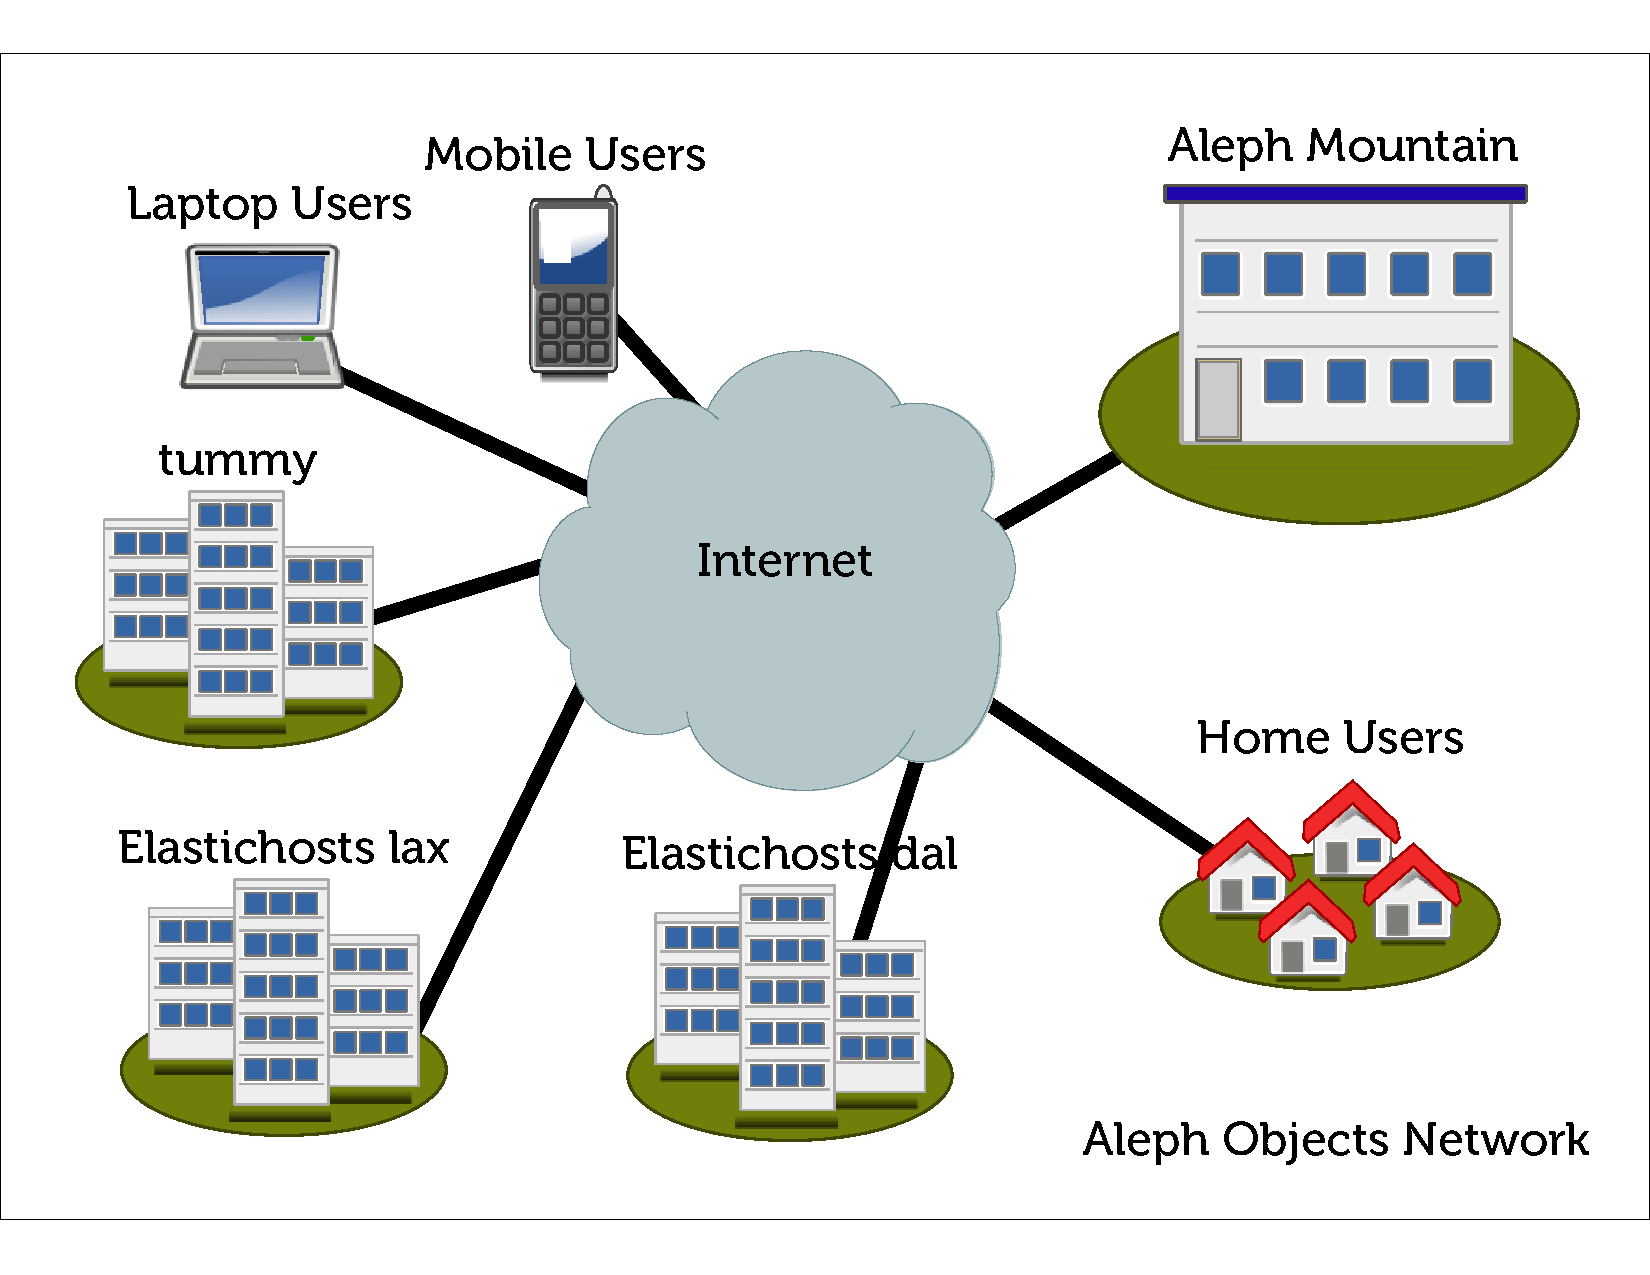
\includegraphics[keepaspectratio=true,height=1.10\textheight,width=1.00\textwidth,angle=0]{ao-network-overview.pdf}
% \caption{Aleph Objects Network Overview}
% \label{fig:ao_net_overview}
%\end{sidewaysfigure}

%\begin{sidewaysfigure}[p]
%\thisfloatpagestyle{empty}
%% The aonet-dot.png built with dot from aonet.dot source.
%
\includegraphics[keepaspectratio=true,height=1.10\textheight,width=1.00\textwidth,angle=0]{aonet-dot.png}
% \caption{Aleph Objects Network Overview, dot}
% \label{fig:ao_net_dot}
%\end{sidewaysfigure}

%\begin{sidewaysfigure}[p]
%\thisfloatpagestyle{empty}
%% The aonet-neato.png built with neato from aonet.dot source.
%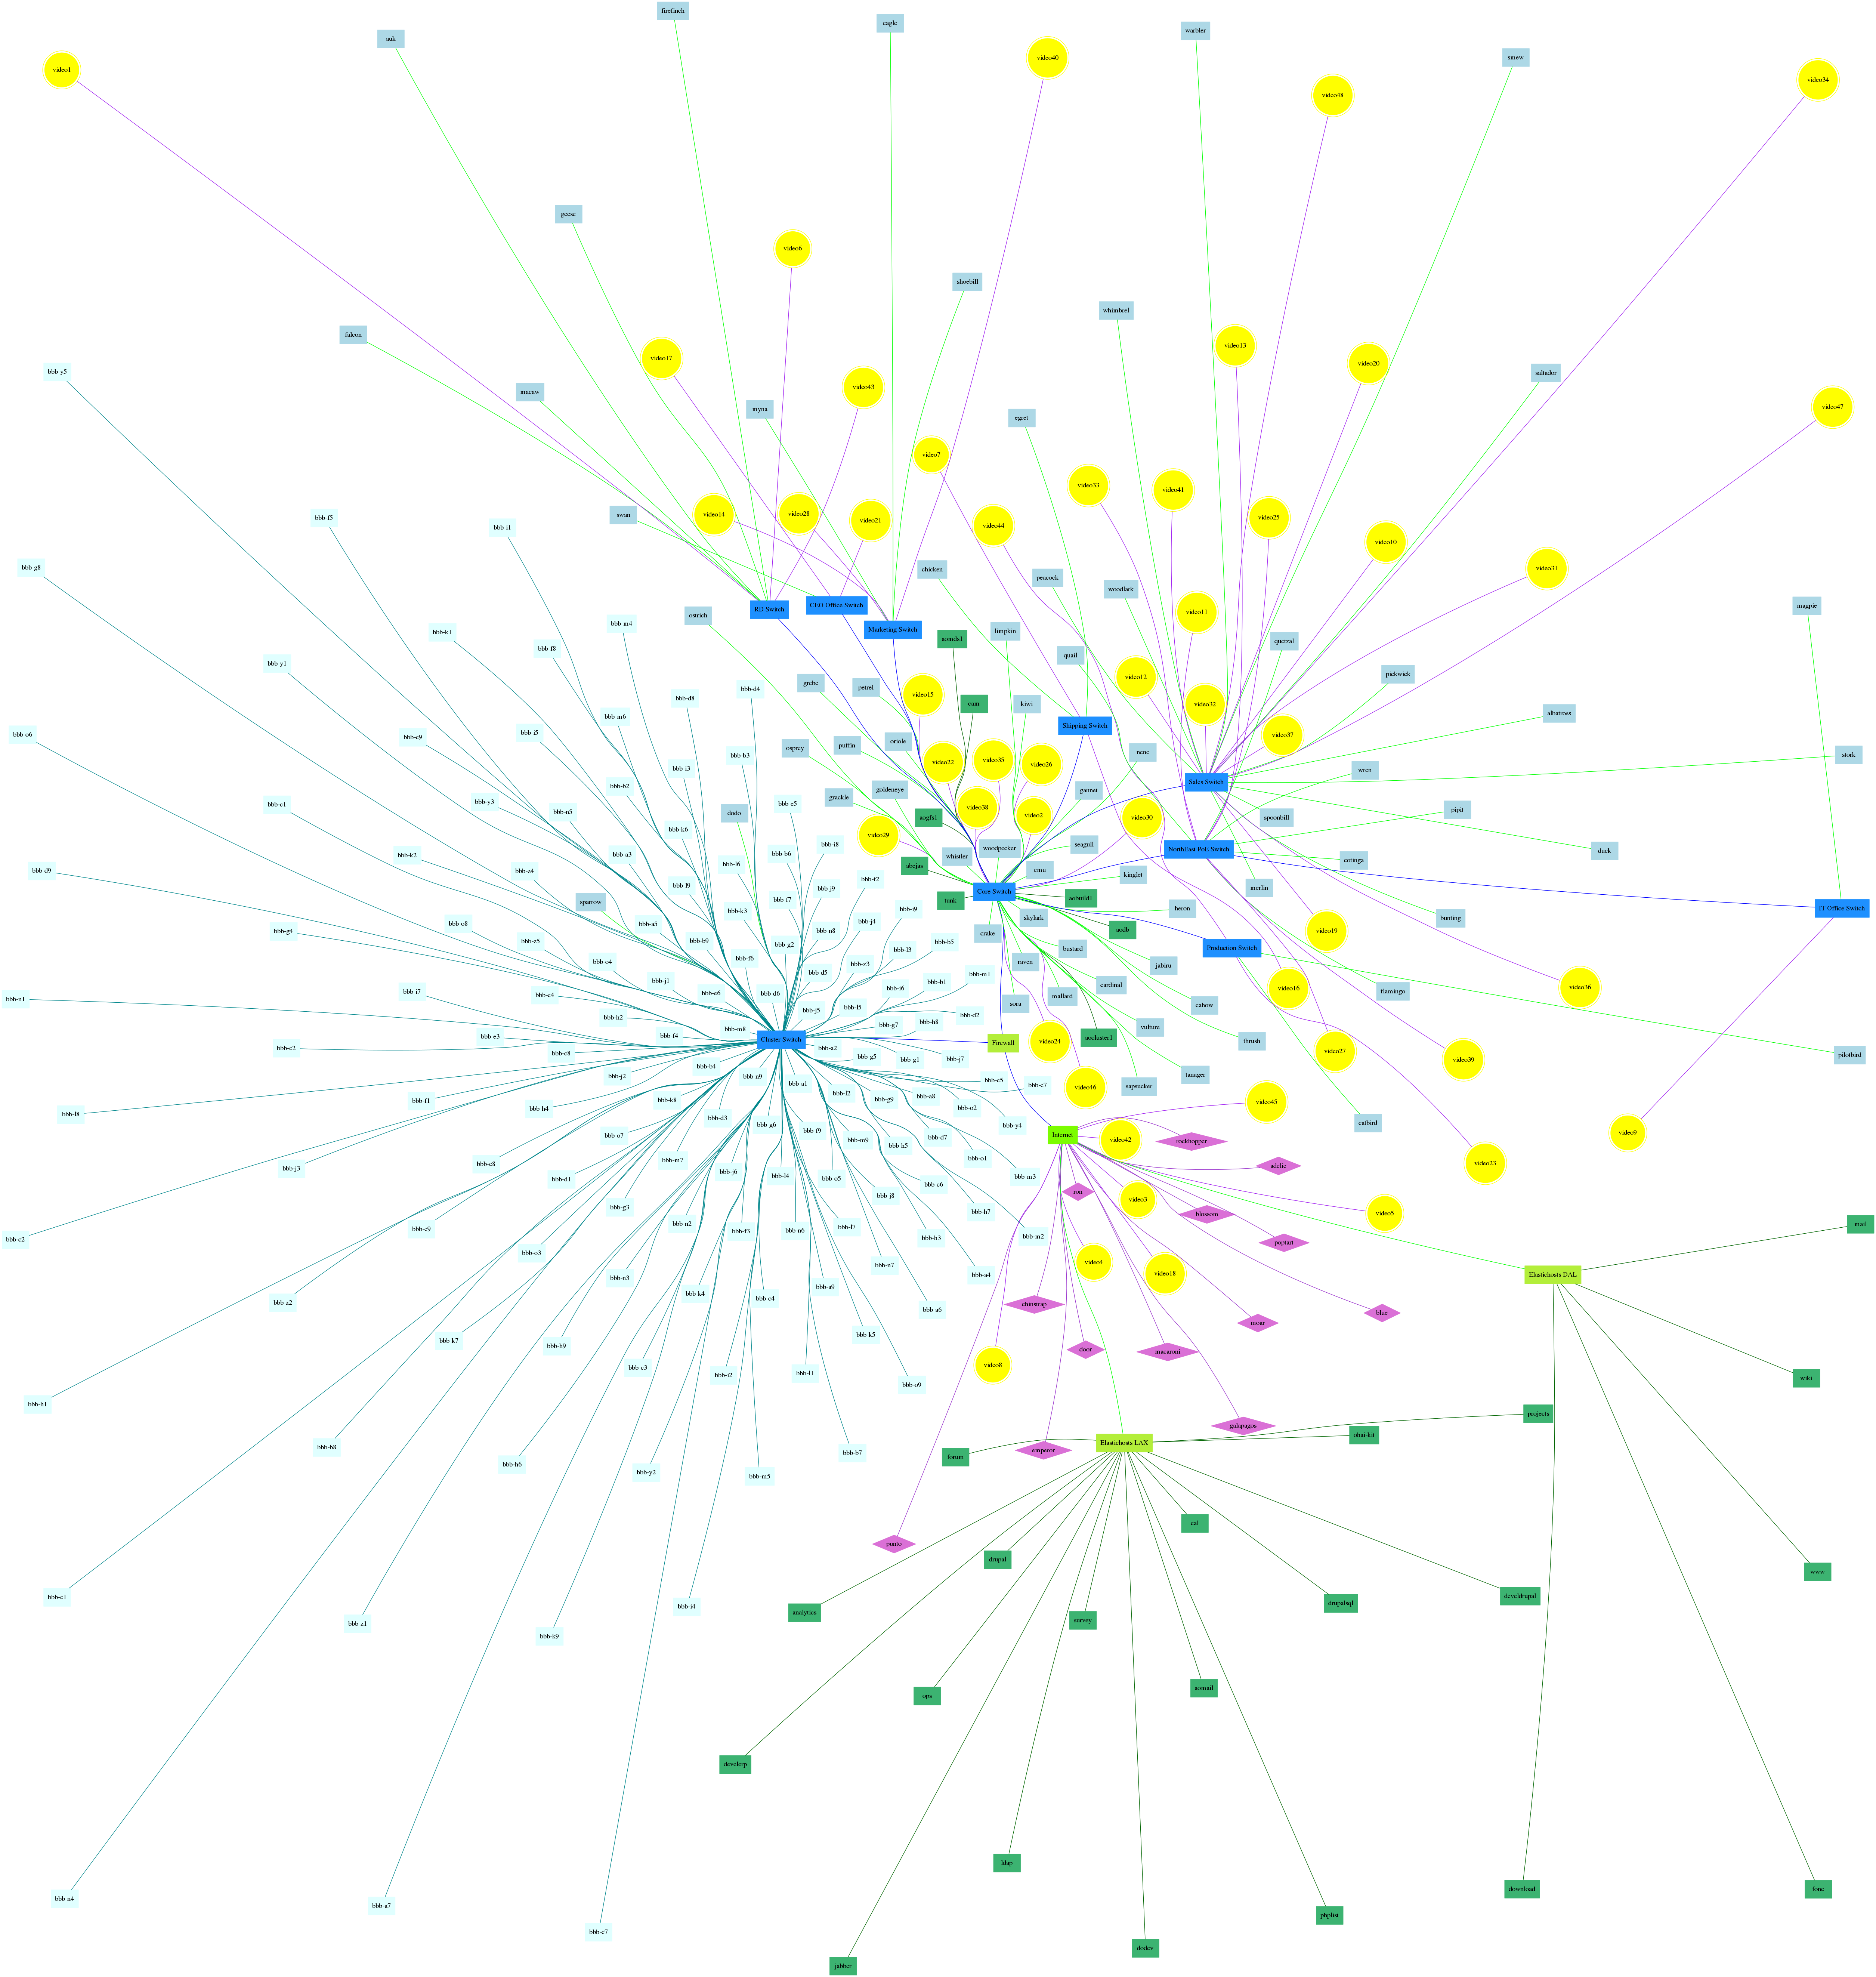
\includegraphics[keepaspectratio=true,height=1.10\textheight,width=1.00\textwidth,angle=0]{aonet-neato.png}
% \caption{Aleph Objects Network Overview, neato}
% \label{fig:ao_net_neato}
%\end{sidewaysfigure}

\begin{sidewaysfigure}[p]
\thisfloatpagestyle{empty}
% The aonet-sfdp.png built with sfdp from aonet.dot source.
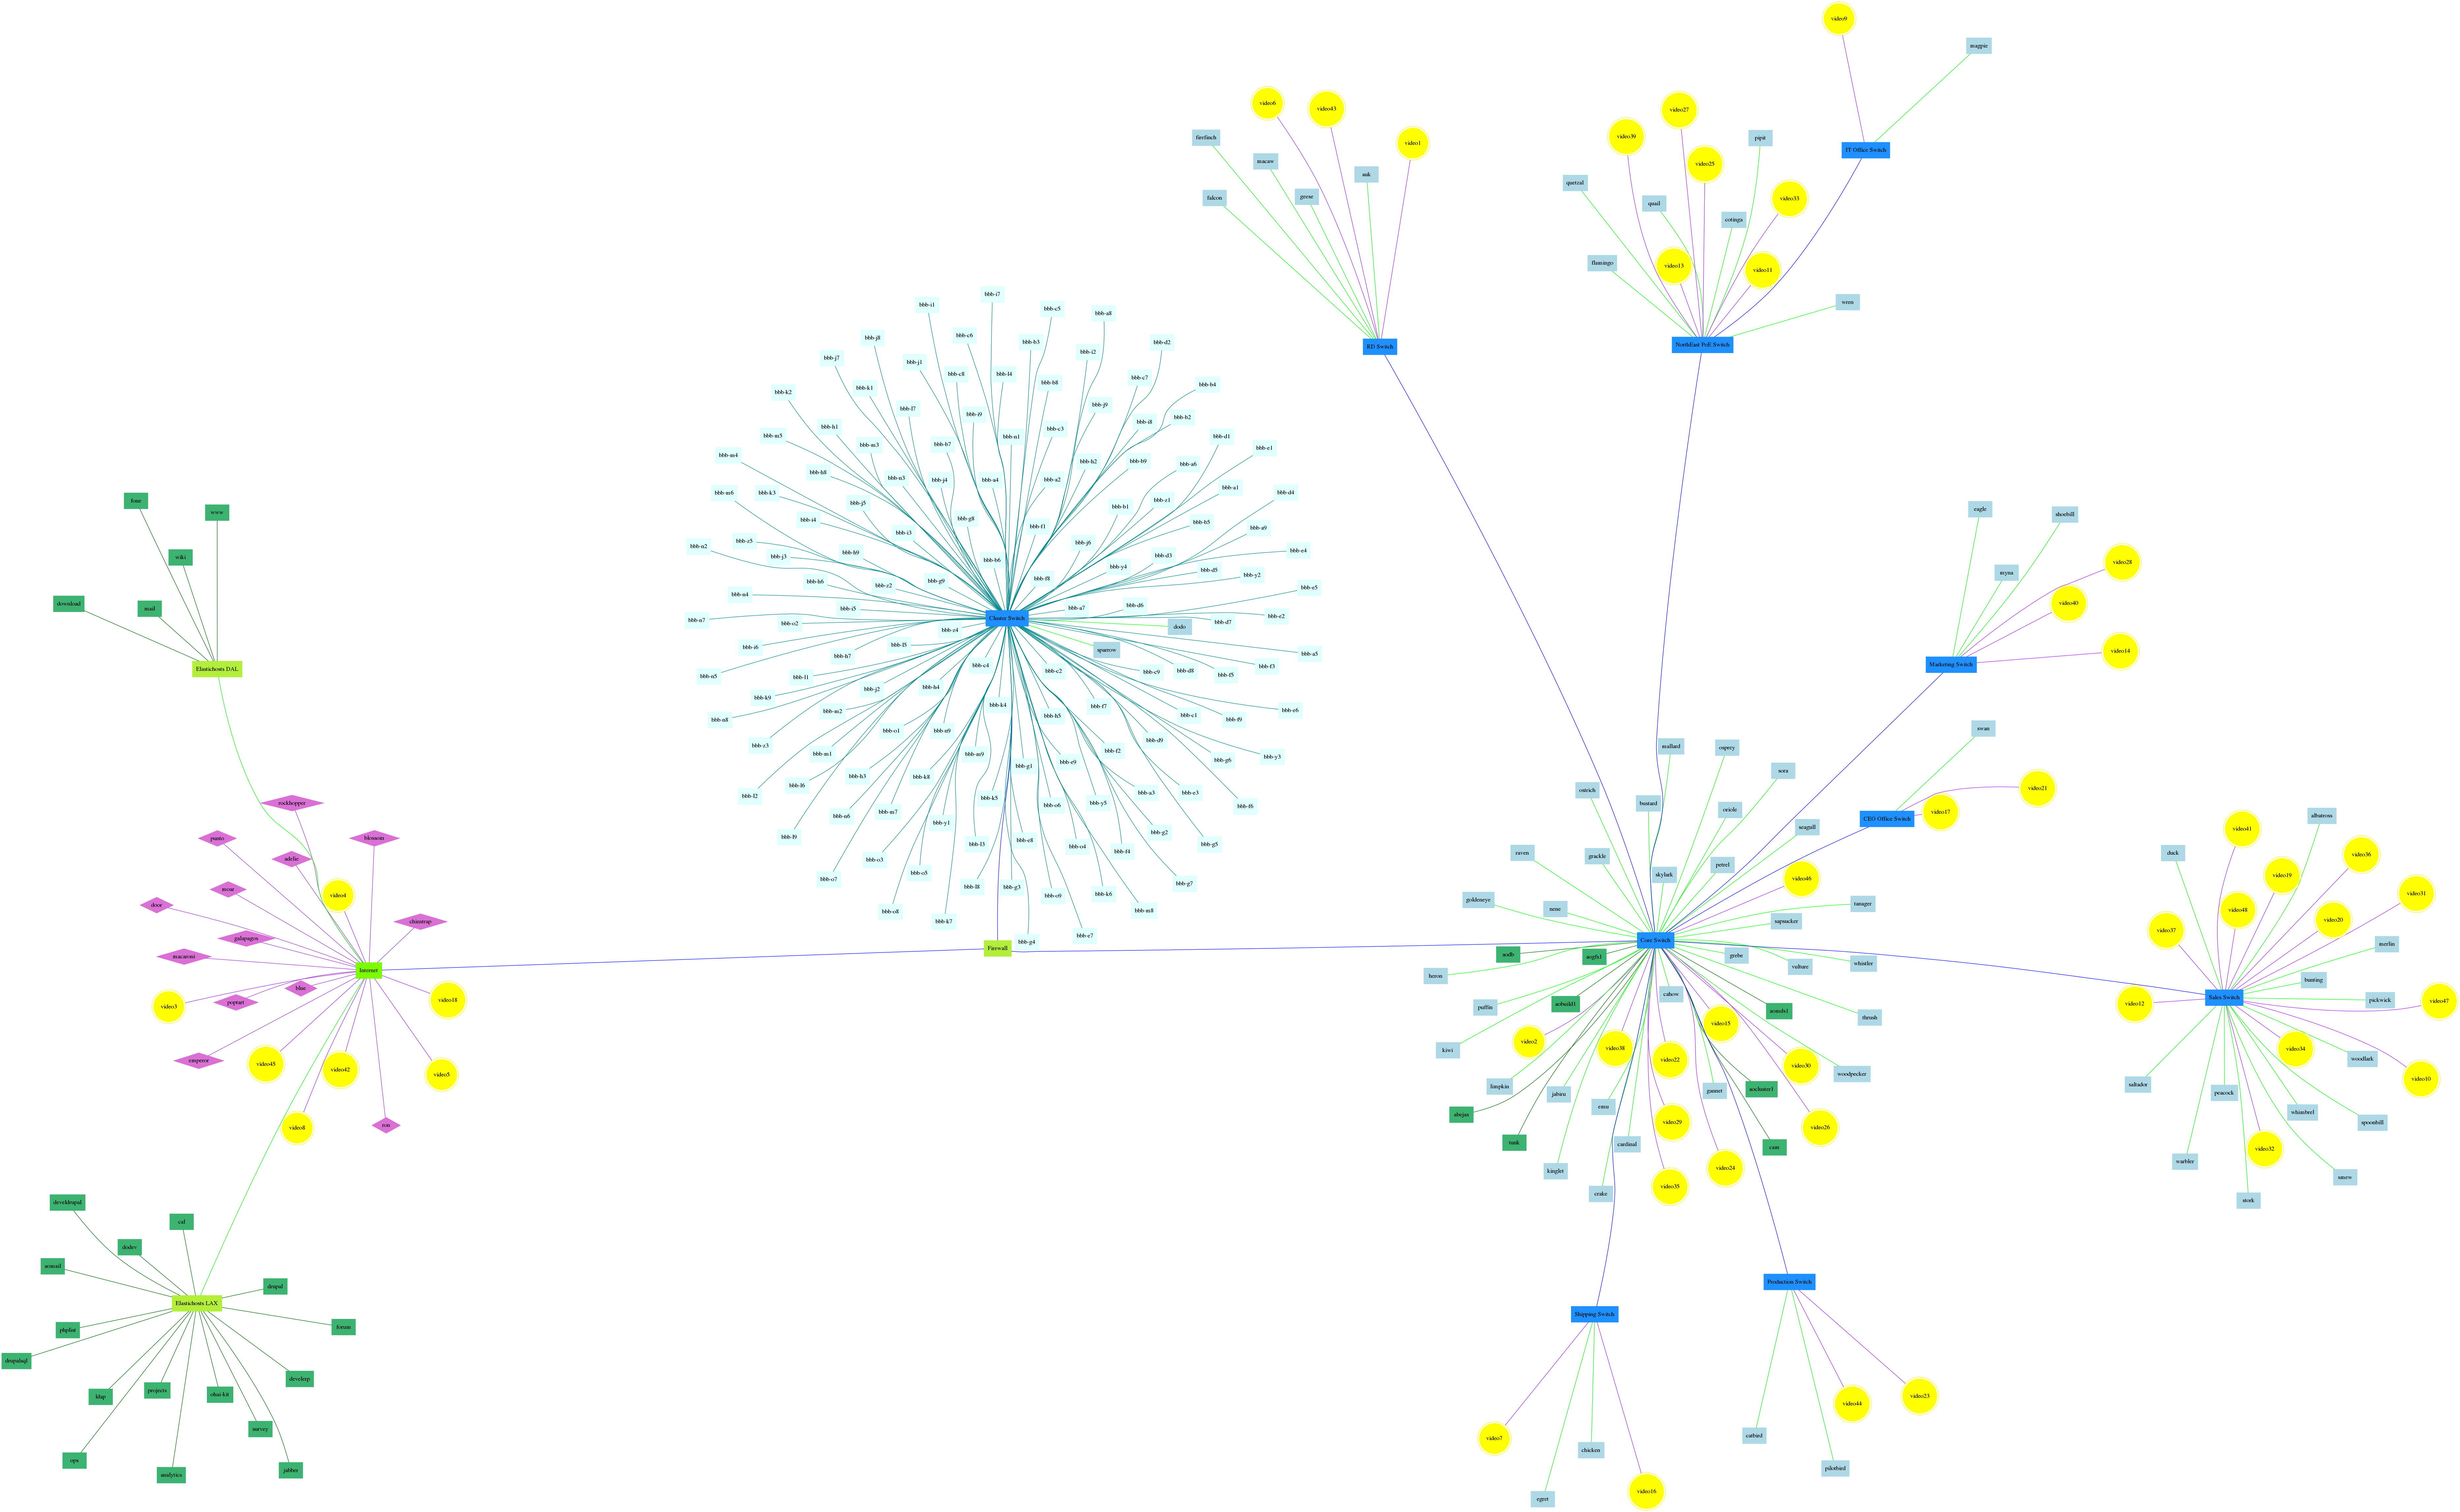
\includegraphics[keepaspectratio=true,height=1.10\textheight,width=1.00\textwidth,angle=0]{aonet-sfdp.png}
 \caption{Aleph Objects Network Detail, May 2015}
 \label{fig:ao_net_sfdp}
\end{sidewaysfigure}

\begin{sidewaysfigure}[p]
\thisfloatpagestyle{empty}
% The ao-network.pdf was built in Dia.
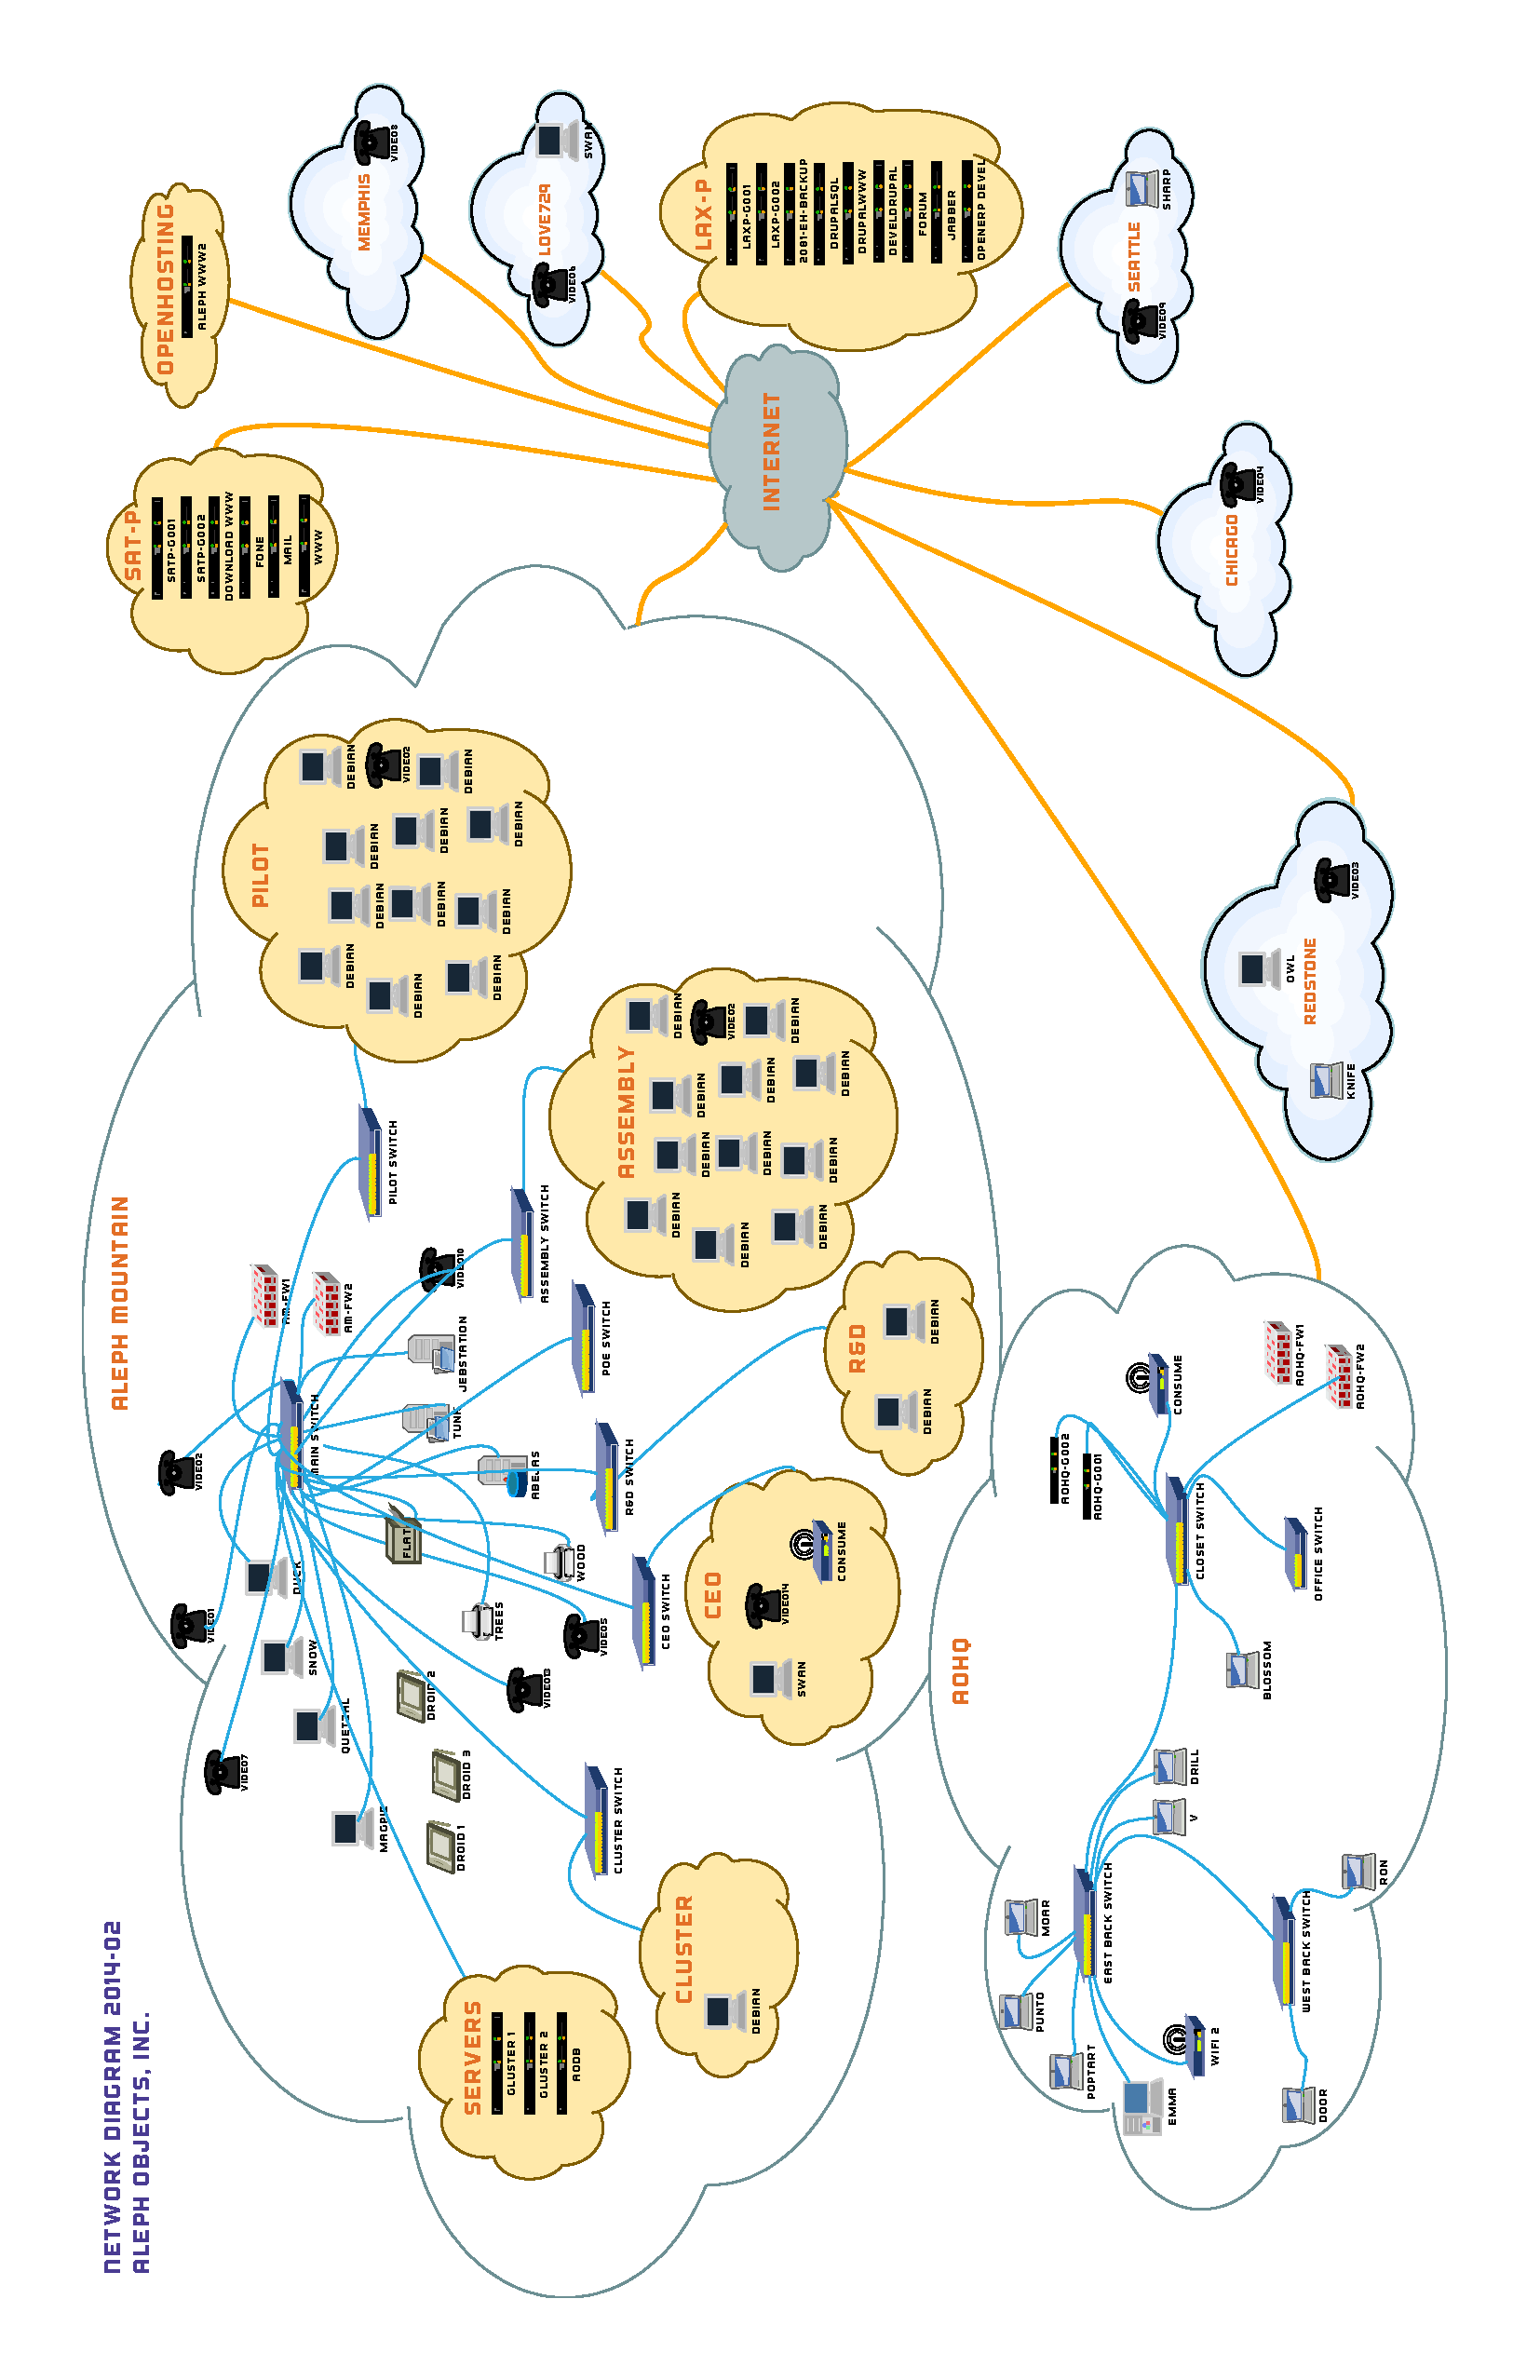
\includegraphics[keepaspectratio=true,height=1.10\textheight,width=1.00\textwidth,angle=-90]{ao-network.pdf}
 \caption{Aleph Objects Network Diagram, February 2014}
 \label{fig:ao_net_dia}
\end{sidewaysfigure}

